\documentclass[11pt]{article}
\usepackage[T1]{fontenc}
\usepackage[utf8]{inputenc}
\usepackage{lmodern}
\usepackage{microtype}
\usepackage[margin=1in]{geometry}
\usepackage{amsmath,amssymb,amsthm,mathtools}
\usepackage{booktabs,longtable,array}
\usepackage{enumitem}
\usepackage{xcolor}
\usepackage{tikz}
\usetikzlibrary{calc,angles,quotes,arrows.meta}
\usepackage{listings}
\usepackage[hidelinks]{hyperref}
\usepackage{url}
\urlstyle{tt}
\allowdisplaybreaks

\definecolor{codebg}{RGB}{247,247,247}
\definecolor{darkblue}{RGB}{20,55,100}
\definecolor{darkgreen}{RGB}{25,100,55}
\lstdefinelanguage{Lean}{
  morekeywords={theorem,lemma,def,structure,namespace,end,section,variable,variables,
    import,where,by,have,calc,let,in,if,then,else,match,with,inductive,instance,
    open,scoped,notation,abbrev,exact,refine,simpa,using,rw,at},
  sensitive=true,
  morecomment=[l]{--},morecomment=[s]{/-}{-/},
  morestring=[b]"
}
\lstset{
  basicstyle=\ttfamily\small,
  backgroundcolor=\color{codebg},
  frame=single,
  breaklines=true,
  columns=fullflexible,
  keepspaces=true,
  showstringspaces=false
}

\newtheorem{theorem}{Theorem}[section]
\newtheorem{lemma}[theorem]{Lemma}
\newtheorem{proposition}[theorem]{Proposition}
\newtheorem{corollary}[theorem]{Corollary}
\theoremstyle{definition}
\newtheorem{definition}[theorem]{Definition}
\newtheorem{remark}[theorem]{Remark}
\newtheorem{construction}[theorem]{Construction}

\newcommand{\iPRA}{\mathsf{iPRA}}
\newcommand{\PR}{\mathsf{PR}}
\newcommand{\Cert}{\mathsf{MorleyCert}}
\newcommand{\EqSq}{\mathsf{EquilateralSq}}
\newcommand{\N}{\mathbb N}
\newcommand{\Q}{\mathbb Q}
\newcommand{\R}{\mathbb R}
\newcommand{\K}{K}
\newcommand{\rotmul}{\mathbin{\odot}}
\newcommand{\sqdist}{\operatorname{sd}}
\newcommand{\im}{\operatorname{im}}
\newcommand{\re}{\operatorname{re}}
\newcommand{\detv}{\operatorname{det}}
\newcommand{\dotp}{\operatorname{dot}}
\newcommand{\code}[1]{\texttt{#1}}

\title{Morley's Trisector Theorem in Intuitionistic Primitive Recursive Arithmetic\\
\large A constructive algebraic proof, an arithmetized certificate theorem, and a Lean completion plan}
\author{Prepared for Vladimir Reshetnikov}
\date{15 November 2026}

\begin{document}
\maketitle

\begin{abstract}
Morley's theorem says that the three intersections of adjacent internal angle
trisectors of a triangle form an equilateral triangle.  A literal formula
quantifying over all real points is not a formula of arithmetic, and the usual
trigonometric proof appears to use real analysis.  This paper gives a precise
constructive replacement suitable for intuitionistic primitive recursive
arithmetic.  A finite exact certificate contains a common polynomial-quotient scalar
representation, algebraic coordinates, unit rotation pairs for the
third-angles, explicit inverse witnesses for every cancellation, positive ray
parameters, and the defining incidence equations.  We define
primitive-recursive predicates
$\Cert(w)$ and $\EqSq(w)$ and prove
\[
   \iPRA\vdash \forall w\,\bigl(\Cert(w)\to\EqSq(w)\bigr).
\]
The geometric proof is the classical short trigonometric argument, but every
sine and cosine is eliminated in favor of polynomial operations on unit pairs.
The law of sines is replaced by a $2\times2$ determinant identity, the law of
cosines by a dot-product expansion, and all cancellations use explicit
inverse witnesses while sign traces select the internal branches.  The two
genuinely nontrivial algebraic
steps are accompanied by exact ideal-membership certificates and a standalone
sparse-polynomial checker.  We also give a module-by-module Lean plan tied to
the current \code{ConciseIPRA} formalization in the ProveIt repository.
\end{abstract}

\begin{center}
\fbox{\begin{minipage}{0.92\textwidth}
\textbf{Status.}  The paper gives a complete human proof and a detailed
metamathematical reduction to a primitive-recursive certificate implication in
$\iPRA$.  The exact polynomial kernel is machine-checked by the included
Python program, which uses neither a CAS nor floating point arithmetic.
\path{MorleyAlgebra.lean} contains candidate no-\code{sorry} Mathlib lemmas;
\path{MorleyIPRAOutline.lean} gives the object-theory implementation plan.
The delivery environment had no Lean executable, so those files were not
compiled.  A literal Lean derivation of the final $\iPRA$ sequent is therefore
not claimed.
\end{minipage}}
\end{center}

\tableofcontents

\section{The statement and the necessary arithmetical reading}

\subsection{The ordinary geometric theorem}
Let $ABC$ be a nondegenerate Euclidean triangle.  At each vertex draw the two
internal rays that divide the vertex angle into three equal parts.  Let
\begin{itemize}[nosep]
\item $R$ be the intersection of the two trisectors adjacent to side $AB$,
\item $P$ be the intersection of the two trisectors adjacent to side $BC$,
\item $Q$ be the intersection of the two trisectors adjacent to side $CA$.
\end{itemize}
Morley's theorem asserts that $PQR$ is equilateral.  This is the usual ``first
Morley triangle'' formulation \cite{MorleyWiki,Bollobas}.

\begin{figure}[ht]
\centering
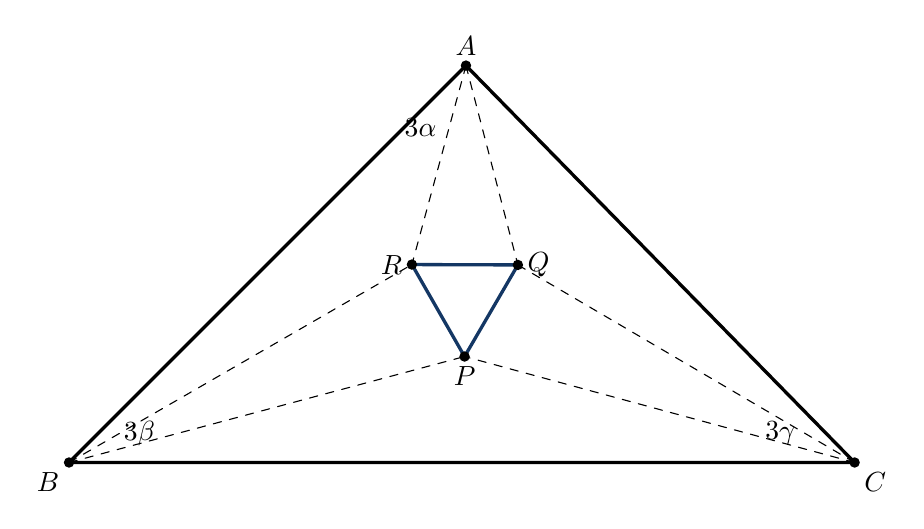
\begin{tikzpicture}[scale=1.05, line cap=round, line join=round]
  \coordinate (A) at (0.3,4.8);
  \coordinate (B) at (-4.5,0);
  \coordinate (C) at (5,0);
  \coordinate (P) at (0.2831,1.2816);
  \coordinate (Q) at (0.9278,2.3893);
  \coordinate (R) at (-0.3538,2.3938);
  \draw[very thick] (A)--(B)--(C)--cycle;
  \draw[thin,dashed] (A)--(R) (A)--(Q) (B)--(R) (B)--(P) (C)--(P) (C)--(Q);
  \draw[very thick,darkblue] (P)--(Q)--(R)--cycle;
  \fill (A) circle (1.8pt) node[above] {$A$};
  \fill (B) circle (1.8pt) node[below left] {$B$};
  \fill (C) circle (1.8pt) node[below right] {$C$};
  \fill (P) circle (1.8pt) node[below] {$P$};
  \fill (Q) circle (1.8pt) node[right] {$Q$};
  \fill (R) circle (1.8pt) node[left] {$R$};
  \node at (-0.25,4.05) {$3\alpha$};
  \node at (-3.65,0.35) {$3\beta$};
  \node at (4.1,0.35) {$3\gamma$};
\end{tikzpicture}
\caption{The labeling used throughout.  Dashed segments lie on the six internal
trisectors; the blue triangle is the first Morley triangle.}
\label{fig:morley}
\end{figure}

\subsection{Why one must state a coded theorem}
The language of $\iPRA$ has natural numbers and primitive-recursive function
symbols, not arbitrary real numbers or points of a continuum.  Consequently,
``for every real triangle'' cannot literally be the matrix of an arithmetical
sentence unless a representation of reals is selected.  There are two honest
ways to express the theorem.

\begin{enumerate}[label=(\roman*)]
\item Prove that a finite formal derivation of the universal ordered-field
statement passes a primitive-recursive proof checker.
\item Quantify over finite codes for exact configurations and prove that every
code satisfying a primitive-recursive Morley verifier also satisfies a
primitive-recursive equilateral verifier.
\end{enumerate}

We use (ii), because it is computationally informative.  The semantic
ordered-field theorem follows at once, while an optional constructor gives
certificates for every coded real-algebraic triangle.

\subsection{The exact object-theory theorem}
A detailed certificate format is given in Section~\ref{sec:certificate}.  For
now it suffices that both predicates below are primitive recursive.

\begin{definition}[Certificate predicate]
$\Cert(w)$ means that $w$ codes one exact scalar quotient
$\Q[X]/(p)$, normalized residue representatives for all scalars, points
$A,B,C,P,Q,R$, side directions, positive lengths, a common sine-law scale,
third-angle rotations, positive ray parameters, and explicit inverses for
all canceled factors.  It also contains finite sign traces selecting the
internal branches.  All quotient-ring equations, inverse equations, signs,
and incidences must pass their primitive-recursive checkers.
\end{definition}

\begin{definition}[Equilateral predicate]
$\EqSq(w)$ means that the same scalar quotient representation verifies
\[
 \sqdist(P,Q)=\sqdist(Q,R)=\sqdist(R,P),
 \qquad
 \sqdist(X,Y):=(X_1-Y_1)^2+(X_2-Y_2)^2.
\]
Using squared distances avoids square roots and is equivalent to ordinary
equilaterality for nonnegative Euclidean lengths.
\end{definition}

\begin{theorem}[Arithmetized constructive Morley theorem]
\label{thm:ipra-main}
There are explicit primitive-recursive predicates $\Cert$ and $\EqSq$ such
that
\[
  \boxed{\quad\iPRA\vdash
  \forall w\bigl(\Cert(w)\to\EqSq(w)\bigr).\quad}
\]
The proof uses intuitionistic logic only.  Its inductions are quantifier-free
inductions used to evaluate bounded lists and sparse polynomials.
\end{theorem}

\begin{remark}
The theorem is witness-parametric: it says that any six rays certified as the
internal trisectors have equilateral adjacent intersections.  This is the
constructively natural content of Morley's theorem.  It does not presuppose a
choice operation selecting a trisector from an arbitrary uncoded real angle.
Section~\ref{sec:existence} explains how to add a primitive-recursive
constructor for coded algebraic triangles.
\end{remark}

\section{A fully constructive human proof}
\label{sec:human-proof}

Let
\[
  \angle A=3\alpha,\qquad
  \angle B=3\beta,\qquad
  \angle C=3\gamma.
\]
Because $ABC$ is nondegenerate and the trisectors are internal,
\[
  \alpha,\beta,\gamma>0,
  \qquad \alpha+\beta+\gamma=60^\circ.
  \tag{2.1}\label{eq:sum}
\]
Write $x^+=x+60^\circ$ and $x^{++}=x+120^\circ$.

\subsection{The one trigonometric factorization}

\begin{lemma}[Shifted triple-angle identity]
\label{lem:triple}
For every $x$,
\[
  \sin(3x)=4\sin x\,\sin(x+60^\circ)\,\sin(x+120^\circ).
  \tag{2.2}\label{eq:triple}
\]
\end{lemma}

\begin{proof}
Put $s=\sin x$, $c=\cos x$, and $\rho=\sqrt3$.  Then
\[
 \sin(x+60^\circ)=\frac{s+\rho c}{2},\qquad
 \sin(x+120^\circ)=\frac{-s+\rho c}{2}.
\]
Hence
\begin{align*}
4s\sin(x+60^\circ)\sin(x+120^\circ)
 &=s\bigl((\rho c)^2-s^2\bigr)\\
 &=s(3c^2-s^2)
 =3s-4s^3
 =\sin(3x).
\end{align*}
Every equality is polynomial after the relations $c^2+s^2=1$ and
$\rho^2=3$ are supplied.  In particular, this proof requires no continuity or
power series.
\end{proof}

\subsection{The two trisector lengths from one vertex}
Let $\lambda$ denote the common sine-law scale of $ABC$; classically
$\lambda=2\mathcal R$, where $\mathcal R$ is the circumradius.  Thus
\[
 AB=\lambda\sin(3\gamma),\quad
 AC=\lambda\sin(3\beta),\quad
 BC=\lambda\sin(3\alpha).
 \tag{2.3}\label{eq:sides}
\]
No circle is needed: these three equations are merely the determinant form of
the sine law, discussed in Section~\ref{sec:determinants}.

In triangle $ABR$, the angles at $A$ and $B$ are $\alpha$ and $\beta$.
Therefore
\[
  \angle ARB=180^\circ-\alpha-\beta=120^\circ+\gamma=\gamma^{++}.
\]
The sine law in $ABR$ gives
\[
  AR\sin\gamma^{++}=AB\sin\beta.
\]
All displayed sines are positive, so constructive cancellation is legitimate.
Using \eqref{eq:sides} and Lemma~\ref{lem:triple},
\begin{align}
 AR
 &=\lambda\frac{\sin(3\gamma)\sin\beta}{\sin\gamma^{++}}
  =4\lambda\sin\beta\sin\gamma\sin\gamma^+.
 \tag{2.4}\label{eq:AR}
\end{align}
Similarly, triangle $ACQ$ has angles $\alpha,\gamma,\beta^{++}$, and hence
\begin{align}
 AQ
 &=\lambda\frac{\sin(3\beta)\sin\gamma}{\sin\beta^{++}}
  =4\lambda\sin\beta\sin\gamma\sin\beta^+.
 \tag{2.5}\label{eq:AQ}
\end{align}
Set
\[
 k:=4\lambda\sin\beta\sin\gamma,
 \qquad x:=\beta^+,
 \qquad y:=\gamma^+.
 \tag{2.6}\label{eq:kxy}
\]
Then $AQ=k\sin x$ and $AR=k\sin y$.  The included angle $\angle QAR$ is the
middle third $\alpha$.

\subsection{The central side}
By the dot-product expansion (the algebraic law of cosines),
\begin{align*}
 RQ^2
 &=AR^2+AQ^2-2(AR)(AQ)\cos\alpha\\
 &=k^2\bigl(\sin^2y+\sin^2x-2\sin x\sin y\cos\alpha\bigr).
 \tag{2.7}\label{eq:coslaw}
\end{align*}
From \eqref{eq:sum},
\[
 x+y=\beta+\gamma+120^\circ=180^\circ-\alpha.
\]
Consequently $\cos\alpha=-\cos(x+y)$ and
$\sin\alpha=\sin(x+y)$.  Now calculate without division:
\begin{align*}
&\sin^2x+\sin^2y-2\sin x\sin y\cos\alpha\\
&\quad=\sin^2x+\sin^2y+2\sin x\sin y\cos(x+y)\\
&\quad=\sin^2x+\sin^2y
   +2\sin x\sin y(\cos x\cos y-\sin x\sin y)\\
&\quad=(\sin x\cos y+\cos x\sin y)^2\\
&\quad=\sin^2(x+y)=\sin^2\alpha.
\tag{2.8}\label{eq:bracket}
\end{align*}
Substitution into \eqref{eq:coslaw} yields
\[
  RQ^2=(4\lambda\sin\alpha\sin\beta\sin\gamma)^2.
  \tag{2.9}\label{eq:RQ}
\]
Cyclically permuting $A,B,C$ gives the identical right-hand side for $PR^2$
and $PQ^2$.  Therefore
\[
  PQ^2=QR^2=RP^2,
\]
which is precisely $\EqSq$.  Since the internal configuration is
nondegenerate, the common side is positive, so the ordinary side lengths are
equal as well.  This proves Morley's theorem.

\begin{remark}[Constructive audit of the human proof]
No step used excluded middle, choice, compactness, completeness of $\R$, or an
inverse trigonometric function.  The only cancellations were by quantities
carrying explicit positive evidence.  Equations \eqref{eq:triple} and
\eqref{eq:bracket} are polynomial consequences of unit-circle equations.
Thus the apparent trigonometry is notation for finite algebra.
\end{remark}

\section{Eliminating trigonometric and metric primitives}
\label{sec:algebraization}

\subsection{Rotation pairs}
For an ordered field $K$, define a rotation pair as $z=(c,s)\in K^2$ with
$c^2+s^2=1$.  Write
\[
 (c,s)\rotmul(d,t):=(cd-st,ct+sd),
 \qquad \overline{(c,s)}:=(c,-s).
\]
These are polynomial operations.  The second coordinate of $z$ plays the role
of $\sin z$, the first the role of $\cos z$, and multiplication is angle
addition.  Associativity, commutativity, and
$z\rotmul\bar z=(1,0)$ are ring identities.

Let $u=(c_{60},s_{60})$ be the positive $60^\circ$ pair, specified by
\[
 2c_{60}=1,\qquad c_{60}^2+s_{60}^2=1,\qquad s_{60}>0.
 \tag{3.1}\label{eq:u60}
\]
Put $\rho:=2\im u$.  From $2\re u=1$ and $u\rotmul\bar u=(1,0)$,
polynomial normalization gives $\rho^2=3$.  Moreover, for every unit pair
$z=(c,s)$,
\[
 2\im(z\rotmul u)=s+\rho c,
 \qquad
 2\im(z\rotmul u^2)=-s+\rho c.
 \tag{3.2}\label{eq:shift-pairs}
\]
Thus the two shifted sines in Lemma~\ref{lem:triple} are literally coordinates
of products of pairs.  A direct polynomial calculation also gives
$u^3=(-1,0)$.  Let $a,b,g$ be the positive one-third rotations at $A,B,C$.
The angle-sum statement is simply
\[
 a\rotmul b\rotmul g=u.
 \tag{3.3}\label{eq:rot-sum}
\]
If $x=b\rotmul u$ and $y=g\rotmul u$, then
\[
 x\rotmul y=b\rotmul g\rotmul u^2
 =\bar a\rotmul u^3=(-\re a,\im a),
\]
where \eqref{eq:rot-sum} was multiplied by $\bar a$.  Hence, entirely
algebraically,
\[
 \re(x\rotmul y)=-\re a,
 \qquad \im(x\rotmul y)=\im a.
 \tag{3.4}\label{eq:sum-pair}
\]
These are exactly the two angle-sum relations used in
\eqref{eq:bracket}.

\subsection{The exact certificate for the triple identity}
To make the finite nature of the argument visible, clear the denominators in
Lemma~\ref{lem:triple}.  Put
\[
 T=3s-4s^3,
 \quad U=c^2+s^2-1,
 \quad H=\rho^2-3.
\]
Then the claimed identity has the following explicit ideal-membership
certificate:
\begin{align}
&2T-(2s)(s+\rho c)(-s+\rho c)\\
&\qquad=-6sU-2sc^2H.
\tag{3.5}\label{eq:triple-cert}
\end{align}
Thus $U=H=0$ implies the identity by substitution and ring normalization.
A proof checker only has to multiply sparse polynomials and compare normalized
coefficient lists.

\subsection{The exact certificate for the cosine-law bracket}
Let
\begin{align*}
 U_x&=c_x^2+s_x^2-1,&
 U_y&=c_y^2+s_y^2-1,\\
 C&=c_xc_y-s_xs_y,&
 S&=s_xc_y+c_xs_y,\\
 H_c&=C+c_\alpha,&
 H_s&=S-s_\alpha.
\end{align*}
The target polynomial is
\[
 E=s_x^2+s_y^2-2s_xs_yc_\alpha-s_\alpha^2.
\]
The complete certificate is
\begin{equation}
 E=-s_x^2U_y-s_y^2U_x-2s_xs_yH_c+H_s(S+s_\alpha).
 \tag{3.6}\label{eq:bracket-cert}
\end{equation}
Consequently $U_x=U_y=H_c=H_s=0$ implies $E=0$.  The included program
\path{verify_morley_identities.py} checks
\eqref{eq:triple-cert}, \eqref{eq:bracket-cert}, and sixteen connecting
identities using exact fractions and a hand-written sparse-polynomial type.

\subsection{Determinants replace the sine law}
\label{sec:determinants}
For vectors $v=(v_1,v_2)$ and $w=(w_1,w_2)$, put
\[
 \detv(v,w)=v_1w_2-v_2w_1.
\]
Suppose two rays meet:
\[
  X+t u=Y+r v.
\]
Taking determinants with $v$ gives
\[
  t\detv(u,v)=\detv(Y-X,v).
 \tag{3.7}\label{eq:det-intersection}
\]
If $u,v$ are unit direction pairs, their determinant is the algebraic sine of
the oriented angle between them.  Equation \eqref{eq:det-intersection} is the
sine law in exactly the form needed for \eqref{eq:AR} and \eqref{eq:AQ}.
There is no division until a positive determinant is canceled, and its
nonzeroness is part of the certificate.

Likewise, for a common origin $X$,
\begin{align}
\sqdist(X+tu,X+rv)
 &=t^2\dotp(u,u)+r^2\dotp(v,v)-2tr\dotp(u,v).
 \tag{3.8}\label{eq:dot-cos}
\end{align}
For unit $u,v$, $\dotp(u,v)$ is the algebraic cosine of the included angle.
Equation \eqref{eq:dot-cos} is a raw polynomial expansion, not a theorem about
square roots.

\subsection{The human proof translated literally into pairs}
The translation contains no hidden analytic step.  Replace
\[
 \sin\alpha,\sin\beta,\sin\gamma
   \quad\text{by}\quad \im a,\im b,\im g,
 \qquad
 \cos\alpha\quad\text{by}\quad\re a,
\]
and replace shifted sines by \eqref{eq:shift-pairs}.  Store a scalar
$\lambda$ satisfying
\begin{align}
 \ell_{BC}&=\lambda\,\im(a^3),&
 \ell_{CA}&=\lambda\,\im(b^3),&
 \ell_{AB}&=\lambda\,\im(g^3).
 \tag{3.9}\label{eq:lambda-pair}
\end{align}
Applying \eqref{eq:det-intersection} to the two incidences defining $R$ and
$Q$, then using \eqref{eq:triple-cert}, gives
\begin{align}
 AR&=4\lambda\,\im b\,\im g\,\im(g\rotmul u),\notag\\
 AQ&=4\lambda\,\im b\,\im g\,\im(b\rotmul u).
 \tag{3.10}\label{eq:pair-lengths}
\end{align}
The canceled factors are $\im(g\rotmul u^2)$ and
$\im(b\rotmul u^2)$; their inverse witnesses are fields of the certificate.
Put $x=b\rotmul u$ and $y=g\rotmul u$.  Equation
\eqref{eq:sum-pair} says
\[
 \re(x\rotmul y)=-\re a,
 \qquad \im(x\rotmul y)=\im a.
\]
Now \eqref{eq:dot-cos} and \eqref{eq:bracket-cert} give
\[
 RQ^2=(4\lambda\,\im a\,\im b\,\im g)^2.
\]
The other two equalities are literal cyclic renamings.  Thus the
trigonometric proof of Section~\ref{sec:human-proof} is a finite derivation in
the language of commutative rings with named inverses; order is used only to
certify that the selected rays are internal.

\section{The finite Morley certificate}
\label{sec:certificate}

This section fixes one concrete coding contract.  Many equivalent encodings
would work; the theorem does not depend on compression details.

\subsection{Concrete exact scalar codes}
To remove any ambiguity about ``exact arithmetic'', fix the following coding.
A certificate contains a monic square-free polynomial $p\in\mathbb Z[X]$ together with a rational interval carrying a finite root-isolation trace.  Every scalar
is a normalized pair $(q,d)$, with $q\in\mathbb Z[X]$ reduced modulo $p$ and
$d>0$, denoting the residue $q/d$ in $\Q[X]/(p)$.  Addition, negation,
multiplication, reduction modulo $p$, and equality of normalized residues are
bounded integer-polynomial algorithms.  Hence their graphs are primitive
recursive.

The proof never needs a global assertion that the quotient is a field.  Each
factor that is canceled comes with a residue $e$ and the checked equation
$d e=1$.  Local invertibility is enough.  Sign information, used only to select
the internal rays, is carried by a finite Sturm/Thom or signed-subresultant
trace.  For an actual real-algebraic configuration, $p$ may be chosen as the
minimal polynomial of a primitive element $\theta$ and the trace includes a
rational isolating interval for $\theta$.  The core equality proof depends
only on quotient-ring normalization and the explicit inverse equations; the
sign layer supplies the intended Euclidean interpretation.

\subsection{Geometric data and equations}
Assume first that $A,B,C$ are counterclockwise.  A certificate stores points
$A,B,C,P,Q,R$ in the coded scalar plane, positive side lengths
$\ell_{AB},\ell_{BC},\ell_{CA}$, a positive common scale $\lambda$,
and unit side directions $e_{AB},e_{BC},e_{CA}$.  It checks
\begin{align*}
 B-A&=\ell_{AB}e_{AB},&
 C-B&=\ell_{BC}e_{BC},&
 A-C&=\ell_{CA}e_{CA}.
\end{align*}
Set $e_{BA}=-e_{AB}$, $e_{CB}=-e_{BC}$, $e_{AC}=-e_{CA}$.

The certificate stores unit rotation pairs $a,b,g,u$ and checks
\begin{align}
 e_{AC}&=e_{AB}\rotmul a^3,
 &e_{BA}&=e_{BC}\rotmul b^3,
 &e_{CB}&=e_{CA}\rotmul g^3,
 \tag{4.1}\label{eq:third-rots}\\
 a\rotmul b\rotmul g&=u,
 &2\re u&=1,
 &u\rotmul\bar u&=(1,0),
 &\im u&>0.
 \tag{4.2}\label{eq:sixty-cert}
\end{align}
It also checks the three redundant but proof-convenient scale equations
\begin{align}
 \ell_{BC}&=\lambda\,\im(a^3),&
 \ell_{CA}&=\lambda\,\im(b^3),&
 \ell_{AB}&=\lambda\,\im(g^3).
 \tag{4.3}\label{eq:scale-cert}
\end{align}
For genuine triangles these follow from the determinant form of the sine law;
storing $\lambda$ makes the arithmetic checker local.

The sign block additionally certifies positivity of the following coordinates:
\[
 \im a,\im b,\im g;\qquad
 \im(a\rotmul u),\im(b\rotmul u),\im(g\rotmul u);\qquad
 \im(a\rotmul u^2),\im(b\rotmul u^2),\im(g\rotmul u^2).
\]
These claims select the internal branches; the explicit inverse equations
justify the cancellations.

The six trisector directions are
\begin{align*}
 d_{AR}&=e_{AB}\rotmul a,& d_{AQ}&=e_{AB}\rotmul a^2,\\
 d_{BP}&=e_{BC}\rotmul b,& d_{BR}&=e_{BC}\rotmul b^2,\\
 d_{CQ}&=e_{CA}\rotmul g,& d_{CP}&=e_{CA}\rotmul g^2.
\end{align*}
Finally, positive parameters witness the adjacent intersections:
\begin{align}
 R&=A+r_A d_{AR}=B+r_B d_{BR},\notag\\
 Q&=A+q_A d_{AQ}=C+q_C d_{CQ},\notag\\
 P&=B+p_B d_{BP}=C+p_C d_{CP},
 \tag{4.4}\label{eq:intersections}
\end{align}
with all six parameters strictly positive.  The code also names inverses for
the two shifted-sine factors canceled in each cyclic local proof and verifies
the corresponding product-with-inverse equations.  The clockwise case is
represented by reversing the orientation bit and conjugating every rotation
pair; the squared-distance conclusion is invariant.

\subsection{Primitive-recursive checkers}
All data are finite lists of natural numbers under a standard pairing code.
Bounded parsing, signed-integer arithmetic, polynomial reduction, residue
normalization, inverse verification, sparse-polynomial normalization, and
finite sign-trace checking are primitive recursive.  Thus there are
primitive-recursive Boolean functions
\[
  \code{morleyCertOK}(w),\qquad \code{equilateralSqOK}(w)
\]
such that
\[
 \Cert(w)\equiv\code{morleyCertOK}(w)=1,
 \qquad
 \EqSq(w)\equiv\code{equilateralSqOK}(w)=1.
\]

\begin{proposition}[Checker correctness]
Inside $\iPRA$, unfolding $\code{morleyCertOK}(w)=1$ yields all equations and
positive-apartness facts used in Sections~\ref{sec:human-proof} and
\ref{sec:algebraization}.  The certificates
\eqref{eq:triple-cert} and \eqref{eq:bracket-cert}, instantiated three times,
yield
\[
 \sqdist(P,Q)=M^2,
 \quad \sqdist(Q,R)=M^2,
 \quad \sqdist(R,P)=M^2,
 \qquad M=4\lambda\,\im(a)\im(b)\im(g).
\]
Therefore $\code{equilateralSqOK}(w)=1$.
\end{proposition}

\begin{proof}
Every inference is one of the following: evaluation of a primitive-recursive
operation, substitution into an equality, ring normalization, determinant or
dot-product expansion, conjunction introduction/elimination, or cancellation
by a factor with a checked multiplicative inverse.  These are intuitionistically valid.  Polynomial and list normalization are
proved by quantifier-free induction on their coded bounds.  Every branch of the
checker is a decidable equality or order comparison of integers, so no case
split on an undecidable proposition occurs.  Repeating the local derivation
for the three cyclic permutations and introducing the universal quantifier
gives the ordinary-$\iPRA$ derivation of Theorem~\ref{thm:ipra-main}.
\end{proof}



\section{Why the proof fits the ProveIt \texorpdfstring{$\iPRA$}{iPRA} kernel}

The current ProveIt \code{ConciseIPRA} development already provides the
logical and proof-theoretic infrastructure required by the plan.  In
particular, \code{PR.lean} defines primitive-recursive symbols \code{PR k},
terms \code{PTm n}, the usual $\iPRA$ axioms \code{PRAAx}, and quantifier-free
induction.  \code{Deduction.lean} defines scoped intuitionistic natural
deduction with equality, while \code{NativeBiInterpretation.lean} proves the
faithfulness bridges \code{native\_iff\_pra} and \code{pra\_iff\_native}.
The repository is pinned here to commit
\code{0bba41d70f061442357cae0f6de055434a33fb09} \cite{ProveIt}.

The intended closed theorem has the Lean shape
\begin{lstlisting}[language=Lean]
theorem ipra_morley_certificate :
  [] |- [PRAAx]
    all (morleyCertOK (var 0) == one -->
         equilateralSqOK (var 0) == one)
\end{lstlisting}
where the ASCII notation above is schematic; the actual repository notation
uses \code{\ensuremath{\vdash}[PRAAx]}, \code{\ensuremath{\doteq}}, and
\code{Fm.all}.  The matrix is quantifier-free after checker unfolding.

There are two equally valid implementation directions.
\begin{enumerate}
\item Prove the theorem in the ordinary \code{PRAAx} presentation and transport
it to the native calculus using \code{pra\_iff\_native}.
\item Build the reflected certificate proof in the native calculus and use
\code{native\_iff\_pra} to obtain ordinary $\iPRA$ derivability.
\end{enumerate}
The second route should produce the smaller final proof object; the first route
is easier to debug.

\section{Existence of certificates for algebraic triangles}
\label{sec:existence}

The core theorem needs no global existence principle: it accepts the six
trisectors and their intersections as witnesses.  For a stronger
computational corollary, suppose $A,B,C$ have real-algebraic coordinates.
Then a certificate can be constructed effectively.

\begin{construction}[Primitive-recursive algebraic constructor]
\begin{enumerate}
\item Compute positive algebraic side lengths by adjoining roots of
$X^2-\sqdist(A,B)$, etc., with rational isolating intervals selecting the
positive roots.
\item Normalize side vectors.  At each vertex solve the fixed-degree system
\[
 z\bar z=1,\qquad z^3=v,
\]
where $v$ is the unit rotation from one side to the other.
\item Use a Sturm or signed-subresultant certificate to select the unique root
inside the relevant oriented sector.  The inequalities are rational sign
queries at real-algebraic numbers.
\item Form the six ray directions and solve three $2\times2$ linear systems.
The determinants are positive by the sector certificates, so the solutions are
unique and have positive parameters.
\item Put all resulting algebraic numbers into one primitive-element
presentation and emit the normalized residues, inverse witnesses, and sign
traces used by $\Cert$.
\end{enumerate}
\end{construction}

All polynomial degrees in the trisection step are fixed.  Standard coefficient
height and root-separation bounds give a primitive-recursive bound on the
number of bisections and on every intermediate code size; signed remainder
sequences are bounded by degree.  Therefore this constructor can be represented
by a \code{PR} symbol.  Formalizing its correctness is a substantial but
separate algebraic-number project.  Once that correctness proof is entered,
it yields the stronger target
\[
 \iPRA\vdash\forall t\bigl(\mathsf{AlgTriangle}(t)
 \to\exists w\,[\mathsf{Builds}(w,t)\wedge\Cert(w)]\bigr).
\]
That target, combined with Theorem~\ref{thm:ipra-main}, gives Morley's theorem
for every triangle whose coordinates are given by finite real-algebraic codes.
The universal theorem over arbitrary real coordinates remains a semantic
consequence of the same ordered-field derivation; arithmetic itself cannot
quantify over uncoded reals.

\section{Lean formalization roadmap}
\label{sec:lean}

The Archive of Formal Proofs contains a 2025 Isabelle development using
complex geometry and Connes's proof \cite{AFP}.  A 2026 Lean development also
proves a geometric complex-plane statement and supplies existence and
nondegeneracy results \cite{UnicoMorley}.  Those are useful API references, but
they rely on real/complex analytic infrastructure.  The proposed formalization
below is deliberately smaller at the trusted mathematical layer: it proves a
finite algebraic certificate theorem and then reflects it into $\iPRA$.

\subsection{Module graph}
\begin{longtable}{>{\raggedright\arraybackslash}p{0.30\textwidth}>{\raggedright\arraybackslash}p{0.62\textwidth}}
\toprule
Module & Main responsibility \\
\midrule
\endhead
\path{Morley/Poly.lean} & Signed integers, sparse polynomials, normalization,
and checking the explicit ideal-membership certificates. \\
\path{Morley/ScalarCert.lean} & Polynomial-quotient residues, normalized
rational denominators, local inverse witnesses, and optional sign traces. \\
\path{Morley/Rot.lean} & Pair multiplication, conjugation, norm, powers,
$u^3=-1$, shifted-coordinate identities, and the algebraic angle-sum lemma. \\
\path{Morley/Vec2.lean} & Dot product, determinant, squared distance,
ray points, determinant intersection lemma, and the two-ray expansion. \\
\path{Morley/Certificate.lean} & Natural-number encoding and the
primitive-recursive Boolean \code{morleyCertOK}. \\
\path{Morley/Core.lean} & Generic proof that a valid certificate has three
equal squared central sides. \\
\path{Morley/PRA.lean} & Reification as \code{PTm}, proof in
\code{Prf PRAAx}, and universal closure. \\
\path{Morley/Native.lean} & Transfer through \code{native\_iff\_pra} or
\code{pra\_iff\_native}; optional compressed native certificate. \\
\path{Morley/Alg.lean} & Optional real-algebraic constructor and root-isolation
correctness. \\
\bottomrule
\end{longtable}

\subsection{First executable milestone}
The first milestone should not mention geometry.  It imports the included
\path{MorleyAlgebra.lean} and proves the two central identities over an arbitrary
linear ordered field:
\begin{lstlisting}[language=Lean]
theorem shifted_triple_angle
    (s c rho : K)
    (hunit : c ^ 2 + s ^ 2 = 1)
    (hrho : rho ^ 2 = 3) :
    4 * s * ((s + rho*c)/2) * ((-s + rho*c)/2)
      = 3*s - 4*s^3 := by
  ...

theorem morley_bracket
    (sx cx sy cy sa ca : K)
    (hx : cx^2 + sx^2 = 1)
    (hy : cy^2 + sy^2 = 1)
    (hcos : cx*cy - sx*sy = -ca)
    (hsin : sx*cy + cx*sy = sa) :
    sx^2 + sy^2 - 2*sx*sy*ca = sa^2 := by
  ...
\end{lstlisting}
The supplied candidate proofs use only \code{ring}, \code{rw}, and
\code{linarith}/\code{nlinarith}.  After this compiles, replace tactic proofs
with the explicit certificates \eqref{eq:triple-cert} and
\eqref{eq:bracket-cert}; that makes reflection into $\iPRA$ direct.

\subsection{Second milestone: generic ordered-field geometry}
Define \code{Rot K := K \ensuremath{\times} K} and \code{Vec2 K := K
\ensuremath{\times} K}.  Prove the determinant and dot-product lemmas without
using \code{Real.angle}, \code{Real.sin}, norms, or square roots.  State a
structure whose fields are exactly equations \eqref{eq:third-rots}--
\eqref{eq:intersections}, then prove
\begin{lstlisting}[language=Lean]
theorem morley_of_certificate
    (d : MorleyData K) (hd : d.Valid) :
    sqDist d.P d.Q = sqDist d.Q d.R /\
    sqDist d.Q d.R = sqDist d.R d.P := by
  ...
\end{lstlisting}

\subsection{Third milestone: reflection and the object theory}
Implement the polynomial-quotient scalar checker and sparse-polynomial
normalizer as \code{PR} symbols.
Prove their defining equations once.  The generic field proof then becomes a
sequence of checker steps, and its closed acceptance trace yields
\code{ipra\_morley\_certificate}.  Apply the existing bi-interpretation theorem
to obtain the corresponding native result.  This is a clear path to a
complete Lean formalization because each boundary has a finite executable
contract and no step depends on an unformalized analytic theorem.

\section{Constructivity and proof-theoretic audit}

\begin{longtable}{>{\raggedright\arraybackslash}p{0.31\textwidth}>{\raggedright\arraybackslash}p{0.61\textwidth}}
\toprule
Potentially nonconstructive-looking step & Constructive replacement \\
\midrule
\endhead
Angles and trigonometric functions & Unit rotation pairs; addition is pair
multiplication and sine/cosine are projections. \\
Law of sines & Determinant equation \eqref{eq:det-intersection}. \\
Law of cosines & Dot-product expansion \eqref{eq:dot-cos}. \\
Division by a sine & Cancellation only after a supplied inverse witness; a sign trace also certifies the internal branch. \\
Choosing a cube root & The core theorem receives the chosen internal root as a
witness; the optional algebraic constructor uses root isolation. \\
Square roots of distances & The conclusion uses squared distances. \\
Equality of algebraic numbers & Equality of normalized polynomial residues modulo the certificate polynomial; decidable and primitive recursive. \\
Sign of an algebraic number & Sturm/Thom or signed-subresultant certificate. \\
Arbitrary real continuum & Semantic model of the universal ordered-field
formula; the arithmetical theorem quantifies only over finite codes. \\
Classical logic & Not used; all implications and conjunctions are proved in
intuitionistic natural deduction. \\
Unbounded search & Not used in the core; optional root isolation has explicit
primitive-recursive degree/height bounds. \\
\bottomrule
\end{longtable}

\section{Claims, limitations, and falsifiability}

\paragraph{Established here.}
The paper gives a complete constructive derivation of equal squared Morley
sides; an explicit finite certificate format; a metamathematical proof that its
checker and conclusion predicate are primitive recursive and that their
universal implication is derivable in $\iPRA$; and exact machine-checked
polynomial certificates for the algebraic kernel.

\paragraph{Not claimed.}
The archive does not contain a completed Lean proof of
\code{ipra\_morley\_certificate}; it contains a detailed completion map and a
candidate Mathlib algebra file.  It does not formalize Sturm theory in the
ProveIt kernel.  It does not claim that $\iPRA$ has an internal type of all real
numbers.  It does not claim straightedge-and-compass constructibility of angle
trisection.

\paragraph{How to falsify the result.}
A counterexample must do one of three things: identify a valid coded
configuration for which the displayed algebraic derivation fails; find a
nonzero residue in an included polynomial certificate; or identify a use of a
principle not derivable in intuitionistic first-order logic plus
quantifier-free induction.  The polynomial-residue claim is directly testable
by the included checker.  Testing the complete object-theory implication is the
purpose of the proposed Lean modules and is not represented as already done.

\section{Further research questions}

\begin{enumerate}
\item Can the full Morley certificate implication be reduced to a single
universal Horn polynomial identity with no explicit order predicates except
branch selection?
\item What is the smallest native \code{ConciseIPRA} proof object for the two
core certificates after full normalization?
\item Can the algebraic-triangle constructor be specialized to fixed-degree
Thom encodings so that no general primitive-element theorem is needed?
\item Is Connes's affine complex identity smaller, after reflection, than the
shifted-triple-angle proof used here, despite its larger human coefficients?
\item Can one formulate and prove the five additional Morley equilateral
triangles in the same certificate language with substantial proof sharing?
\item What fragment weaker than full $\iPRA$ suffices?  The fixed certificate
trace plausibly needs only elementary function arithmetic, while the uniform
list checker uses quantifier-free induction.
\end{enumerate}

\appendix
\section{Standalone verification artifact}
Run
\begin{lstlisting}
python3 verify_morley_identities.py
\end{lstlisting}
from the archive directory.  A successful run prints the number of verified
identities and rewrites \path{morley_identity_certificate.json}.  The script
implements sparse polynomial addition, multiplication, exponentiation, exact
rational coefficients, canonical serialization, and SHA-256 digests.  It does
not import SymPy, NumPy, Sage, or a solver.

The JSON file records eighteen checks:
\begin{enumerate}[nosep]
\item the shifted triple-angle and Morley bracket certificates;
\item $\rho^2=3$ and the $60^\circ/120^\circ$ coordinate-shift formulas;
\item the real and imaginary parts of $u^3=-1$;
\item associativity, commutativity, and conjugate/norm identities for pairs;
\item both coordinates of the algebraic angle-sum reduction
$(b u)(g u)=-\bar a$;
\item determinant extraction from a ray-incidence equation;
\item the two-ray squared-distance expansion and final local-side
factorization.
\end{enumerate}

\section{Suggested repository placement}
A natural destination is
\begin{verbatim}
Geometry/Morley/ConstructiveIPRA/
\end{verbatim}
with the Lean object-theory files under
\begin{verbatim}
Logic/PrimitiveRecursiveArithmetic/ConciseIPRA/Lean/ConciseIPRA/Morley/
\end{verbatim}
The present archive is self-contained and does not modify the repository.

\begingroup
\raggedright
\begin{thebibliography}{9}
\bibitem{MorleyWiki}
Wikipedia contributors,
\emph{Morley's trisector theorem}, accessed 15 November 2026.
\url{https://en.wikipedia.org/wiki/Morley%27s_trisector_theorem}

\bibitem{Bollobas}
B. Bollob\'as,
\emph{The Art of Mathematics: Coffee Time in Memphis},
Cambridge University Press, 2006, pp.~126--127.

\bibitem{Connes}
A. Connes,
\emph{A new proof of Morley's theorem},
algebraic/complex proof commonly circulated as ``Morley's Redux''.

\bibitem{AFP}
B. Puyobro,
\emph{Morley's Theorem}, Archive of Formal Proofs, 7 March 2025.
\url{https://isa-afp.org/entries/Morley_Theorem.html}

\bibitem{UnicoMorley}
Solarys431,
\emph{Morley's Trisector Theorem---an independent geometric formalization in
Lean}, \code{UnicoProofs/Morley.lean}, repository revision
\code{794568d279e377c34e3ab93a5e0626467f7d9e0d}, 2026.
\url{https://github.com/Solarys431/unico-lean-proofs}

\bibitem{ProveIt}
V. Reshetnikov,
\emph{Concise presentations of intuitionistic primitive recursive arithmetic},
ProveIt repository, revision
\code{0bba41d70f061442357cae0f6de055434a33fb09}, 2026.
\url{https://github.com/VladimirReshetnikov/ProveIt/tree/main/Logic/PrimitiveRecursiveArithmetic/ConciseIPRA}

\bibitem{BPR}
S. Basu, R. Pollack, and M.-F. Roy,
\emph{Algorithms in Real Algebraic Geometry}, 2nd ed., Springer, 2006.
\end{thebibliography}
\endgroup

\end{document}
